% Introductory chapter of the thesis


\section{Section title}
\lipsum[1]

Citing some works \cite{strogatz2001exploring, singer2013natural}. 

Showing some maths 
\begin{equation}
    \boldsymbol{u}^* = \boldsymbol{u}/U, \boldsymbol{x}^* = \boldsymbol{x}/L, \mathrm{and} \; p^* = p /(\mu U/L)  \; \mathrm{or}  \;  p/\rho U^2,
\end{equation}
where $U, L$ are characteristic velocity and length scales, respectively.


\section{Another section }


\subsection{Subsection}

\lipsum[1]

Here is a figure
\begin{figure}
\centering
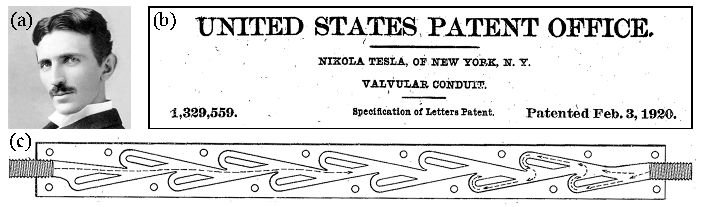
\includegraphics[width=16.5cm]{figures/ch_introductory/fig1.pdf}\vspace{-0.2cm}
\caption{(a) The genius Nikola Tesla (b) His patent (c) Tesla's channel }
\label{fig:chintro-patent}
\end{figure}
 

\subsection{Another subsection}
\lipsum[1]

Here is a table
\ref{table:all-eqs}. 

\begin{landscape}


\begin{table}
    \centering
   \begin{tabular}{ |c|c|>{\centering\arraybackslash}m{5cm}|>{\centering\arraybackslash}m{3cm}| } 
 \hline
 Equations & Initial-boundary value problem &  Applicability &  Under ($\boldsymbol{u},p) \mapsto (-\boldsymbol{u}, -p+c(t))$\\ 
 \hline
 Stokes & \begin{tabular}{@{}c@{}}$    \nabla p - \mu\nabla^2 \boldsymbol{u} = 0$ \\  $\nabla \cdot \boldsymbol{u} = 0 $, \\ with boundary conditions \end{tabular} &  Re $ \ll 1$. The solution is exact near rigid boundaries \cite{childress2009introduction}.   & Reversible  \\ 
 \hline
  Navier-Stokes  & \begin{tabular}{@{}c@{}} $ \rho \left[ \partial \boldsymbol{u}/\partial t + (\boldsymbol{u} \cdot \nabla) \boldsymbol{u} \right] =  -\nabla p + \mu \nabla^2 \boldsymbol{u}$  \\  $\nabla \cdot \boldsymbol{u} = 0$, \\ with initial and boundary conditions \end{tabular} &  Re $> 1$ & Irreversible  \\ 
 \hline
 Euler's &   \begin{tabular}{@{}c@{}} $\partial \boldsymbol{u}/\partial t + (\boldsymbol{u} \cdot \nabla) \boldsymbol{u}  =  -\nabla p$ \\ $\nabla \cdot \boldsymbol{u} = 0$, \\ with initial and boundary conditions \end{tabular}  &  Re$\gg 1$, in free flow regions \cite{batchelor2000introduction}. & Irreversible   \\ 
 \hline
\end{tabular}
    \caption{The governing equations of fluid flow at different dynamical regimes and kinematic (ir)reversibility}
    \label{table:all-eqs}
\end{table}


\end{landscape}  


% \begin{landscape}
% % table
% \end{landscape}

